\chapter{Практическая часть}
\label{cha:ch_2}

\section{Проектирование архитектуры}
% Какая задача поставлена
На основе данной задачи выделяются следующие подзадачи, которые необходимо
выполнить, для успешной реализации инфраструктуры:
\begin{enumerate}[label=\arabic*.]
    \item Описать возможные процессы взаимодействия между компонентами системы.
        Удобно произвести описание с помощью UML диаграммы;
    \item Смоделировать архитектуру приложения: какие компоненты будут
        взаимодействовать друг с другом;
    \item Далее равнозначные задачи, которые не обязательно выполнять
        последовательно: написать файлы запуска и написать кодовую базу для
        запуска каждой из компоненты системы.
\end{enumerate}

Далее рассмотрим каждый из пунктов подробнее, опишем способ реализации,
возникшие проблемы и пути решения.

\section{UML диаграмма}
Для наглядной демонстрации ожидаемого поведения удобно использовать подвид UML диаграмм -- диаграмму активностей.
\begin{figure}[H]
    \centering
    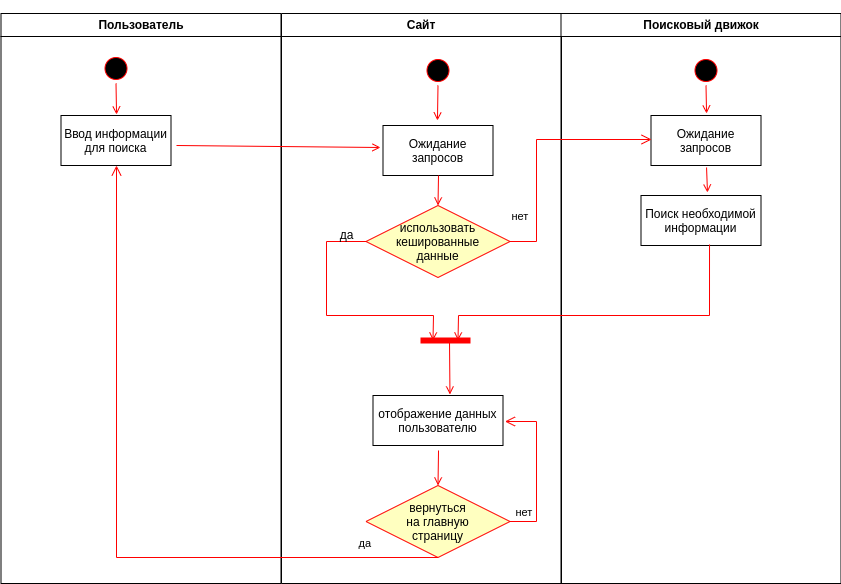
\includegraphics[scale=0.55]{inc/img/activity_diagram.png}
    \caption{Диаграмма активностей для проекта}
\end{figure}

С помощью данной диаграммы можно донести общую концепцию инфраструктуры. Также
на ее основании можно выбрать необходимые для реализации компоненты. Диаграмма
не является точным техническим заданием, а лишь выполняет демонстративную роль.

\section{Архитектура приложения}
После составления UML диаграммы можно определить свойства компонентов и
произвести их выбор.

Для наглядности составим архитектуру всего приложения.
\begin{figure}[H]
    \centering
    
\includegraphics[scale=0.70]{inc/img/structure.png}
    \caption{Архитектура приложения}
\end{figure}

В качестве web-сервера выбран Nginx с его "event based" моделью обработки
входящих соединений, которая обеспечивает быстродействие.

Web-фреймворком выступает Flask, который достаточно легковесный и позволяет
разработчику иметь больше контроля над проектом. Для того, чтобы использовать
Flask вместе с Nginx используется uwsgi.

% TODO: можно еще много чего написать про scrapy и scrapyd: что конкретно
% делают, что конкретно упрощают
Scrapy помогает разработчику извлечь необходимые данные с web-сайтов. Данный
фреймворк написан на Python и имеет открытый исходный код. Содержит в себе
большое количество настроек и достаточно масштабируем "из коробки". В
совокупности со scrapyd позволяет распологать инфраструктуру по поиску на
вычислительных серверах, а также использовать API для просмотра данных.

Для обеспечения доставки сообщений используется kafka (и его модель
Publish-Subscribe). Данный брокер сообщений снимает с приложений нагрузку
связанную с маршрутизацией и отправкой сообщений. Для оркестрации кластеров
kafka используется zookeeper.

В качестве СУБД выбран elasticsearch, т.к. им удобно пользоваться через API
запросы передавая json структуры. Можно создать несколько реплик обеспечив
отказоустойчивость системы. Где каждый узел кластера действует как координатор
для делегирования операций правильному сегменту с автоматической
перебалансировкой и маршрутизацией. Сама СУБД является документоориентированной
что избавляет разработчика от составления схем хранения, хотя для
оптимизированной работы нужно индексировать документы (без схем происходит
автоматически). При продвинутом использовании можно подключить остальные
компоненты системы, например Logstash для работы с логами.

\section{Разработка практических решений}
\subsection{Docker}
\subsection{Docker Compose}
\subsection{Scrapy}
\subsection{Scrapyd}
\subsection{Flask}
\subsection{Kafka}
\subsection{Zookeeper}
\subsection{Kafka Connect}
\subsection{Elastic Search}
